% !TeX spellcheck = pl_PL-Polish
\documentclass[11pt, xcolor={dvipsnames,svgnames},aspectratio=169]{beamer}
\usepackage{lipsum}
\usepackage{amssymb}

\usetheme{iitisask}
\title[]{Perceptron}
\author{Przemysław Głomb}
\date{redaktor pomocniczy: Bartłomiej Gardas}

\theoremstyle{plain}
\newcommand{\scaly}{0.7}

\begin{document}


\frame{\maketitle}

\begin{frame}
	\frametitle{Neuron}
	\begin{center}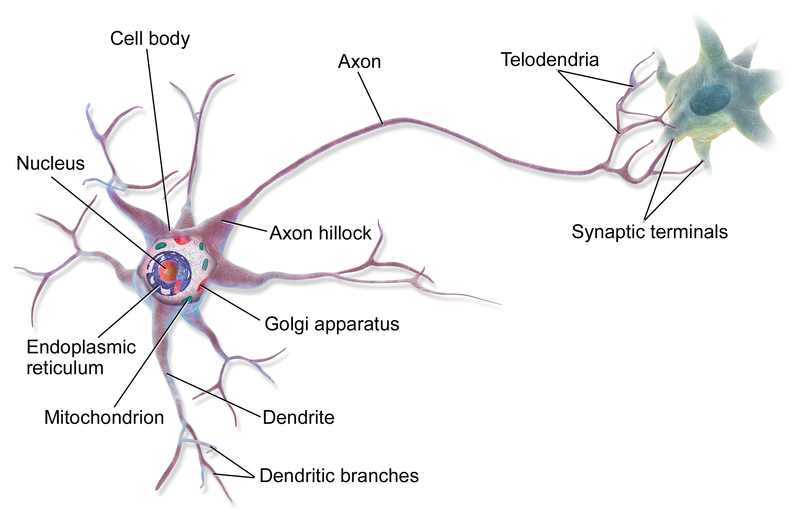
\includegraphics[width=0.6\textwidth]{images/Blausen_0657_MultipolarNeuron.png}\end{center}
	{\tiny https://en.wikipedia.org/wiki/File:Blausen\_0657\_MultipolarNeuron.png, User:BruceBlaus, CC 3}
\end{frame}
\begin{frame}
	\frametitle{Sztuczny neuron (perceptron)}
	\begin{center}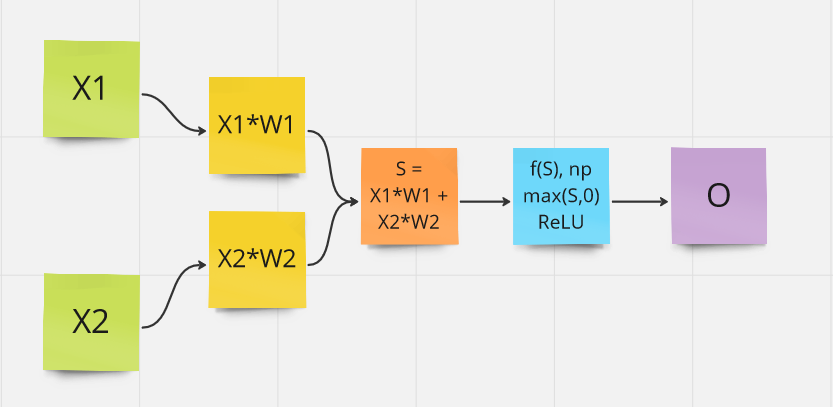
\includegraphics[width=0.8\textwidth]{images/perceptron.png}\end{center}
\end{frame}
\begin{frame}
	\begin{center}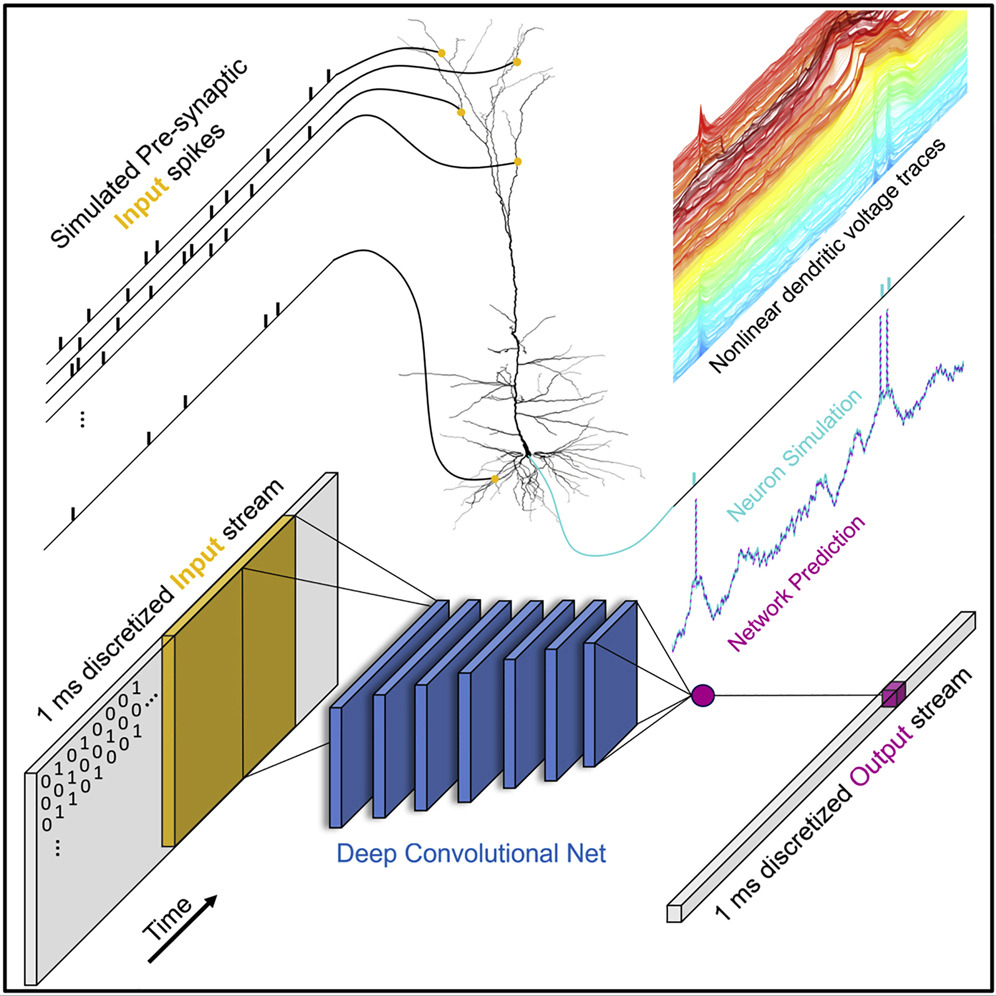
\includegraphics[width=0.45\textwidth]{images/bvsa.jpg}\end{center}
	{\tiny D. Beniaguev, I. Segev, M. London, Single cortical neurons as deep artificial neural networks, Neuron, Volume 109, Issue 17, 2021, Pages 2727-2739.e3,}
\end{frame}
\section{Przykład (,,toy example'') owoce}
\begin{frame}
	\begin{center}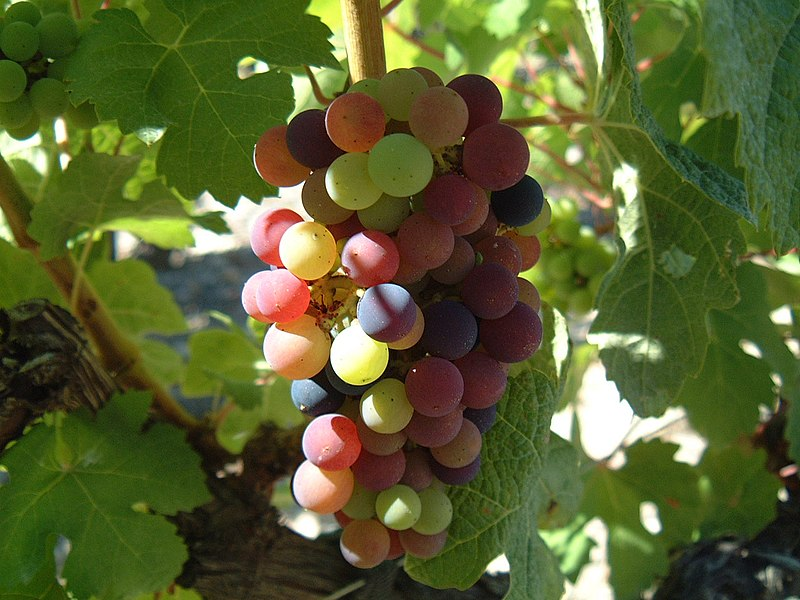
\includegraphics[width=0.5\textwidth]{images/800px-Veraison_Cabernet_Sauvignon.jpg}\end{center}
	{\tiny https://en.wikipedia.org/wiki/File:Veraison\_Cabernet\_Sauvignon.jpg, User:Dominique Hessel, CC 3}
\end{frame}
\begin{frame}
	\begin{center}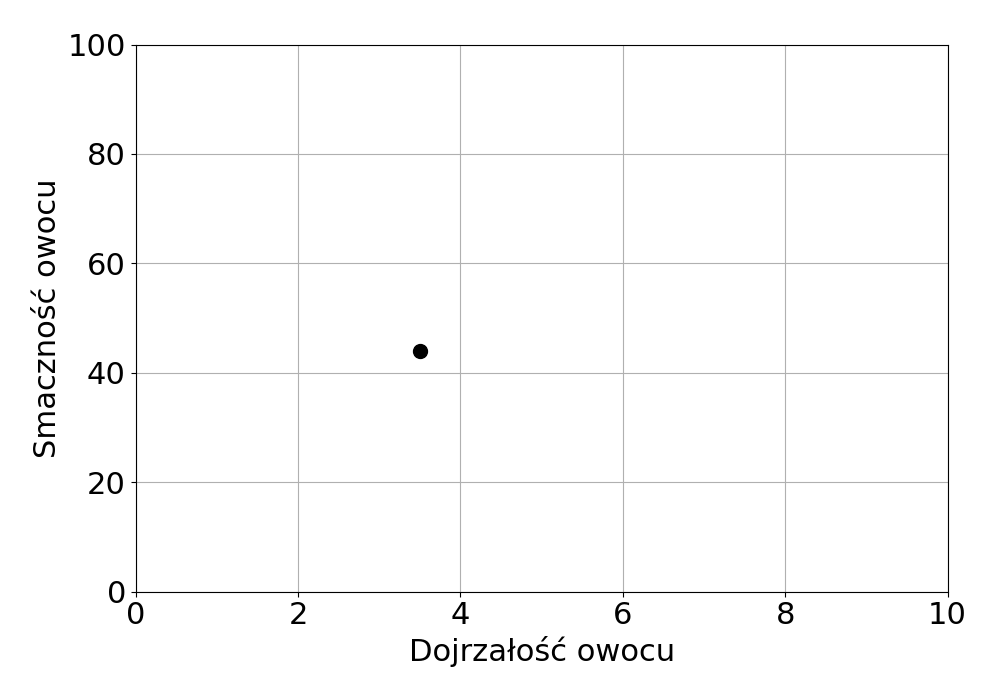
\includegraphics[width=\scaly\textwidth]{images/fruit01.png}\end{center}
\end{frame}
\begin{frame}
	\begin{center}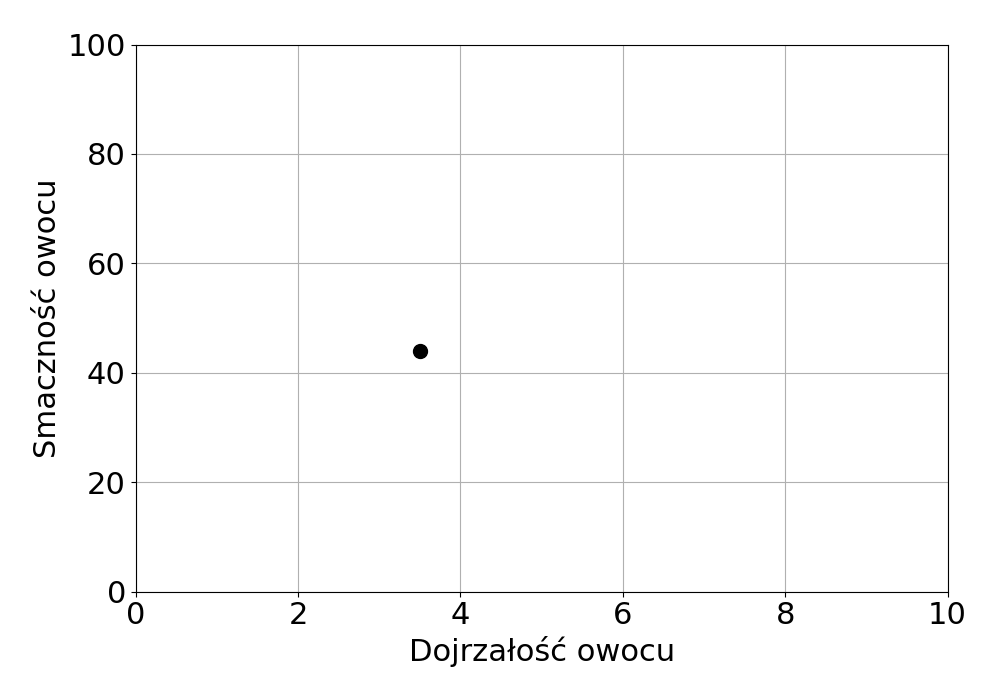
\includegraphics[width=0.3\textwidth]{images/fruit01.png}\end{center}
	$y = f(wx + b)$, $x$ dojrzałość, $y$ smaczność
	\vskip 0.1cm
	np. $f(a)=\max(a, 0)$ (ReLU), $f(a)=\frac{1}{1+e^{-a}}$ (sigmoid), $f(a)=\frac{(e^a - e^{-a})}{(e^a + e^{-a})}$  (tanh)
\end{frame}
\begin{frame}
	\begin{center}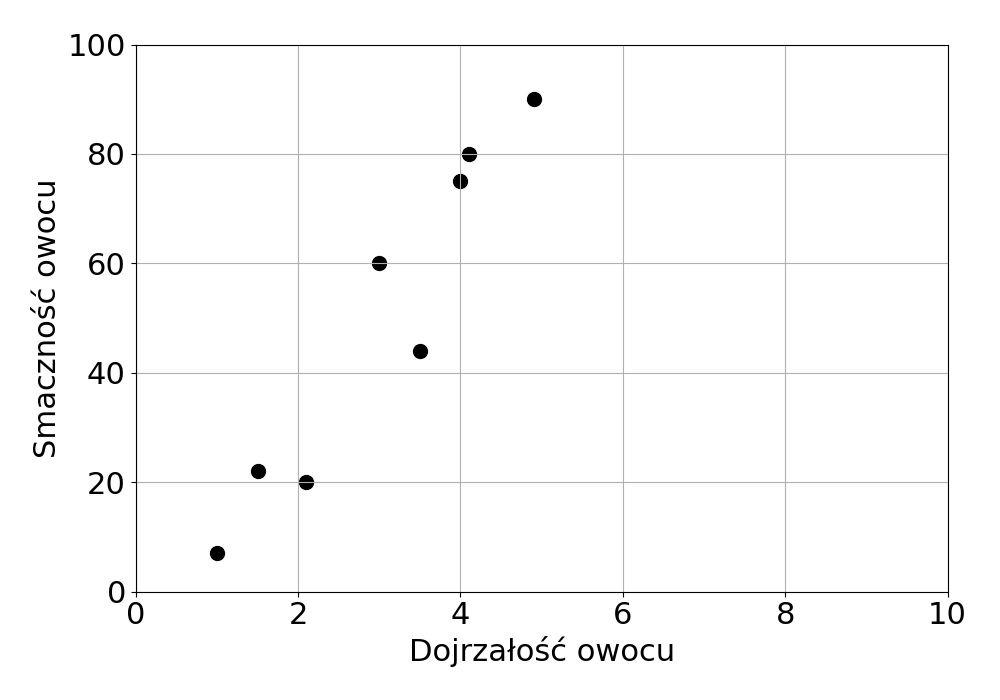
\includegraphics[width=\scaly\textwidth]{images/fruit02.png}\end{center}
\end{frame}
\begin{frame}
	\begin{center} $y = 20x$ \end{center}
	\begin{center}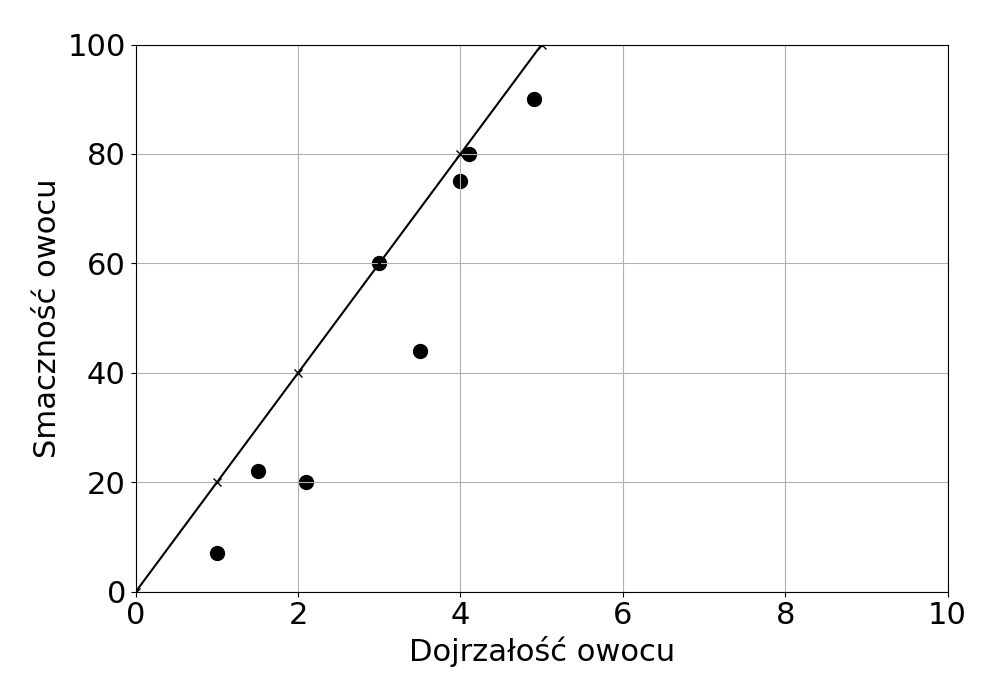
\includegraphics[width=\scaly\textwidth]{images/fruit03.png}\end{center}
\end{frame}
\begin{frame}
	\begin{center} $y = \max(20x - 10, 0)$ \end{center}
	\begin{center}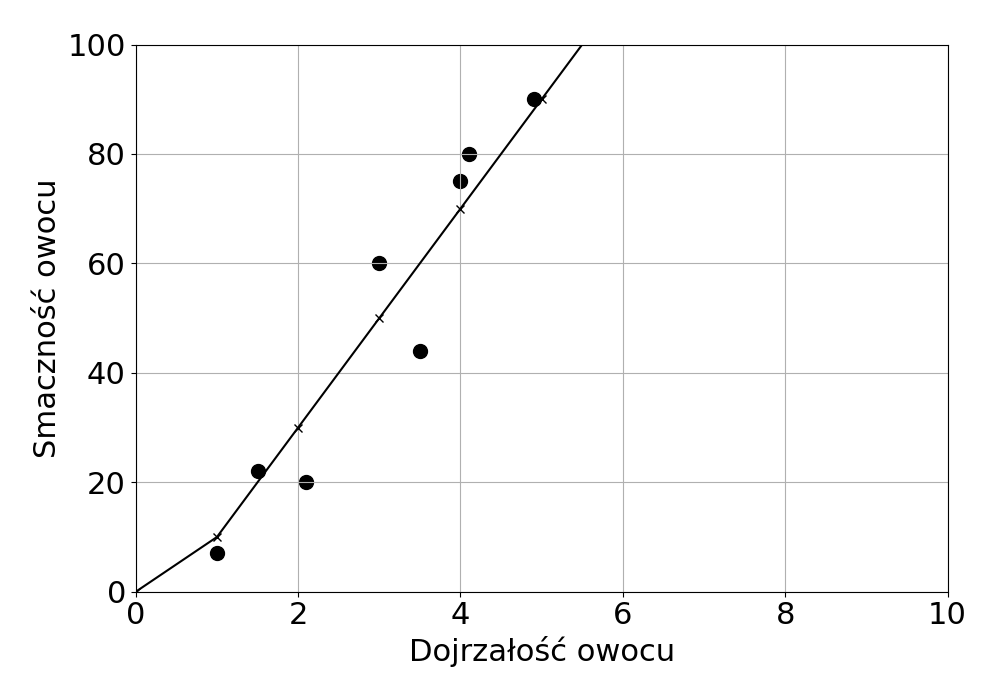
\includegraphics[width=\scaly\textwidth]{images/fruit04.png}\end{center}
\end{frame}
\begin{frame}
	\begin{center} $y = \max(20x - 10, 0)$ \end{center}
	\begin{center}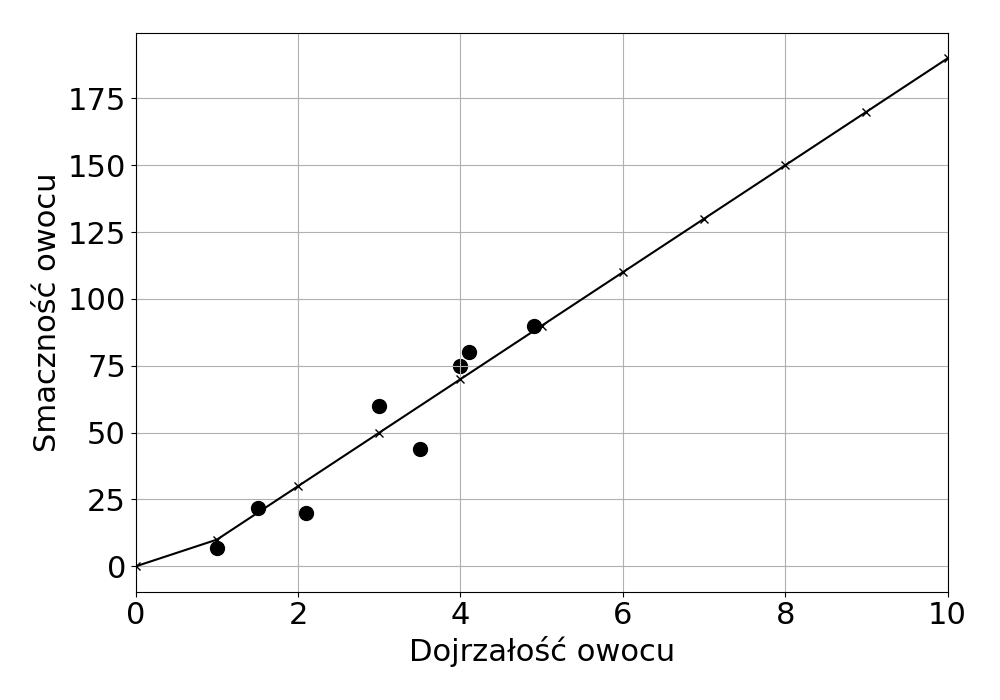
\includegraphics[width=\scaly\textwidth]{images/fruit05.png}\end{center}
\end{frame}
\begin{frame}
	\begin{center} $y = \max(20x - 10, 0)$ \end{center}
	\begin{center}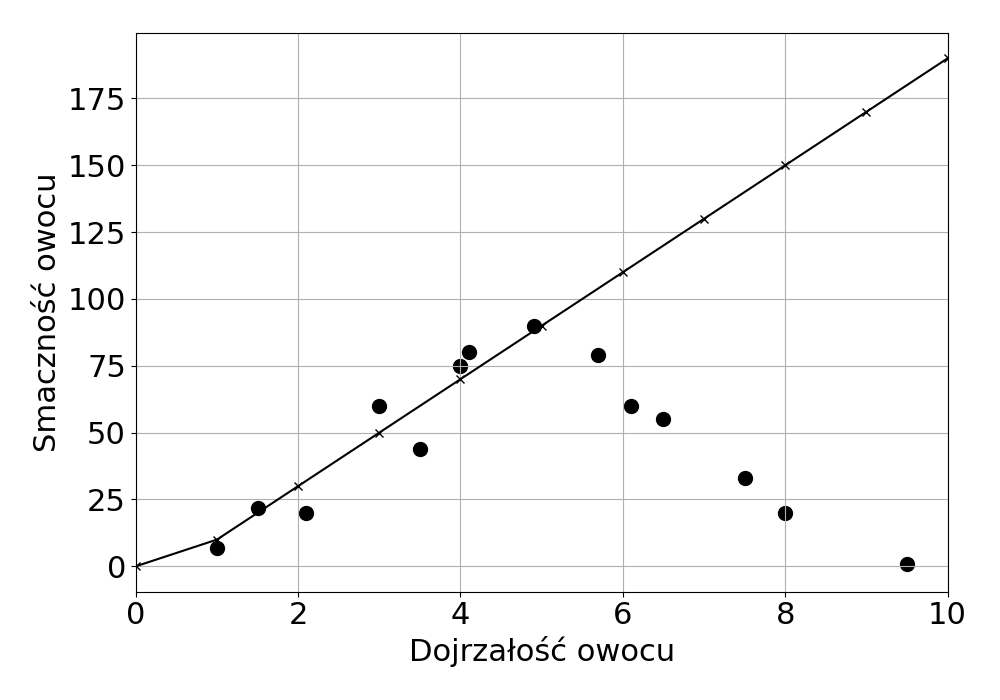
\includegraphics[width=\scaly\textwidth]{images/fruit06.png}\end{center}
\end{frame}
\begin{frame}
	\begin{center} $y = \max(20x - 10, 0)\quad y_2 = \max(40x - 200, 0)$ \end{center}
	\begin{center}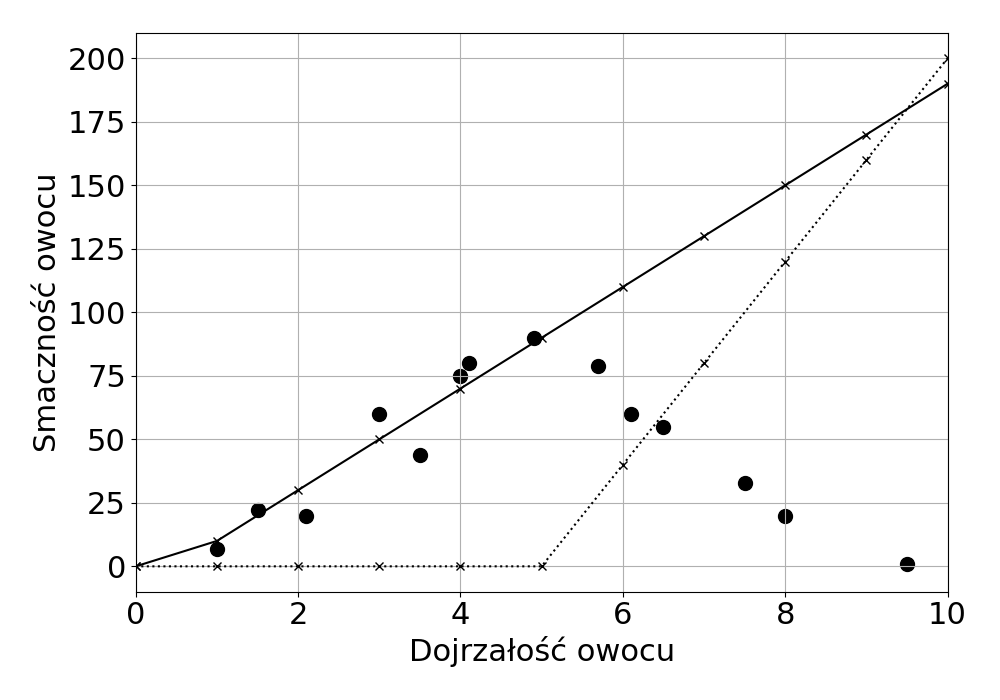
\includegraphics[width=\scaly\textwidth]{images/fruit07.png}\end{center}
\end{frame}
\begin{frame}
	\begin{center} $y = \max(20x - 10, 0)\quad y_2 = \max(40x - 200, 0)$\\$y_{\text{out}} = \max(y - y_2, 0)$ \end{center}
	\begin{center}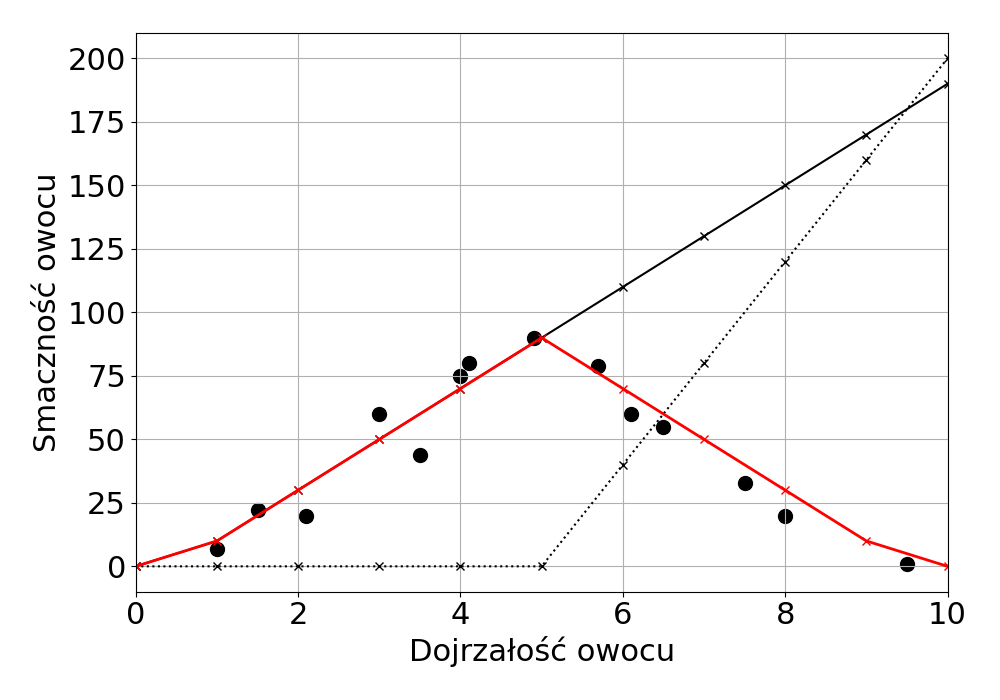
\includegraphics[width=0.6\textwidth]{images/fruit08.png}\end{center}
\end{frame}
\begin{frame}
	\begin{center} $y = \max(20x - 10, 0)\quad y_2 = \max(40x - 200, 0)$\\$y_{\text{out}} = \max(y - y_2, 0)$ \end{center}
	\begin{center}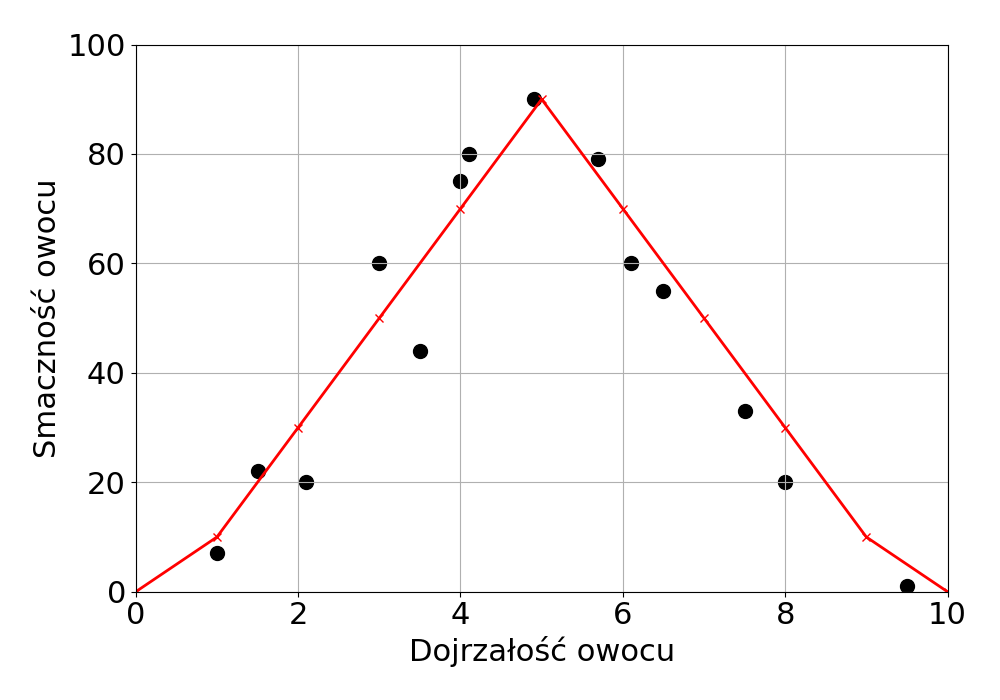
\includegraphics[width=0.6\textwidth]{images/fruit09.png}\end{center}
\end{frame}
\begin{frame}
	\begin{center} $y = \max(20x - 10, 0)\quad y_2 = \max(40x - 200, 0)$\\$y_{\text{out}} = \max(1y - 1y_2 + 0, 0)$ \end{center}
	\begin{center}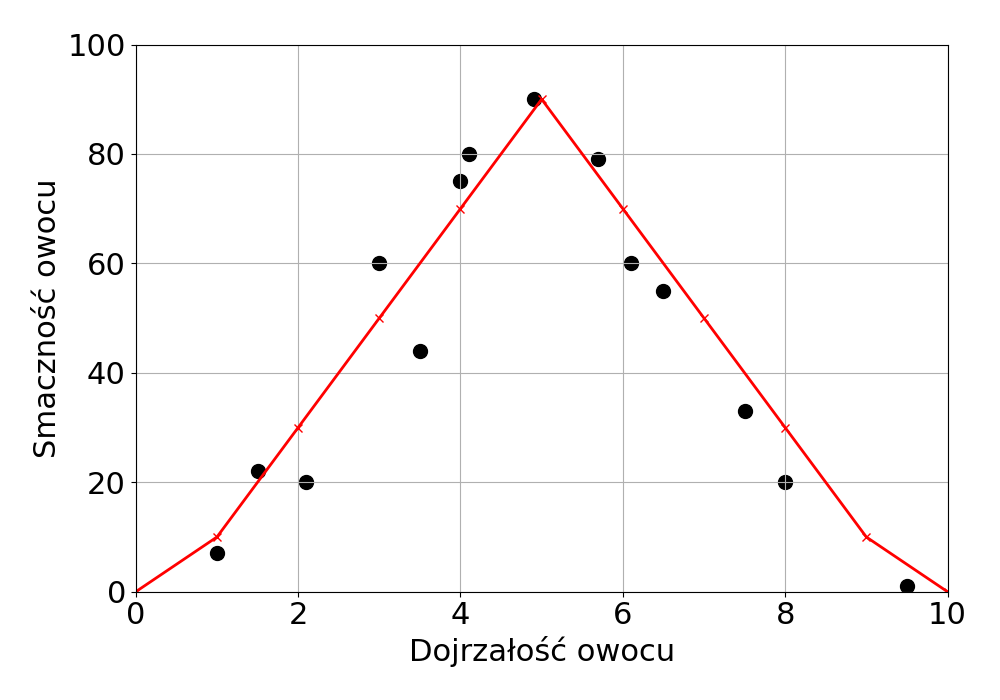
\includegraphics[width=0.3\textwidth]{images/fruit09.png}\end{center}
	\begin{description}
		\item[wynik] działa :)\\
		$x \rightarrow y\qquad x \rightarrow y_2$\\
		$y \rightarrow y_{\text{out}} \leftarrow y_2$
		\item[model] architektura (schemat połączeń neuronów) oraz\\
		wagi $(20, -10, 40, -200, 1, -1, 0)$
		\item[dodatkowo] zbiór danych / model dopasowany do zbioru danych; hierarchie cech
	\end{description}
\end{frame}

\section{Hierarchie cech}

\begin{frame}\begin{center}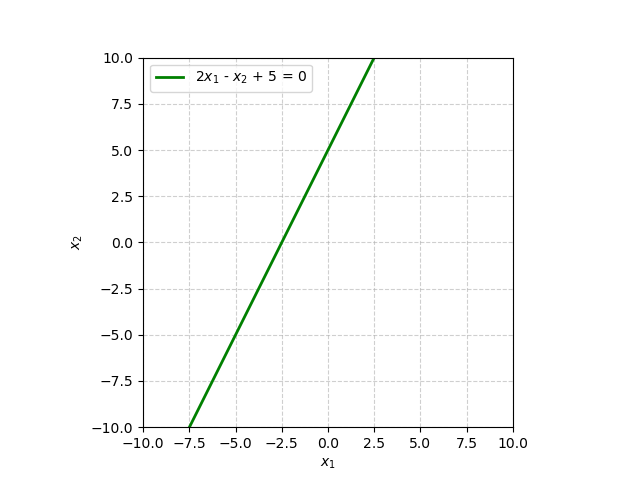
\includegraphics[width=\scaly\textwidth]{images/line.png}\end{center}\end{frame}

\subsection{Jeden neuron wyjściowy, $\circledast\circledast \rightarrow \circledcirc$} % \circleddash 

\begin{frame}\begin{center}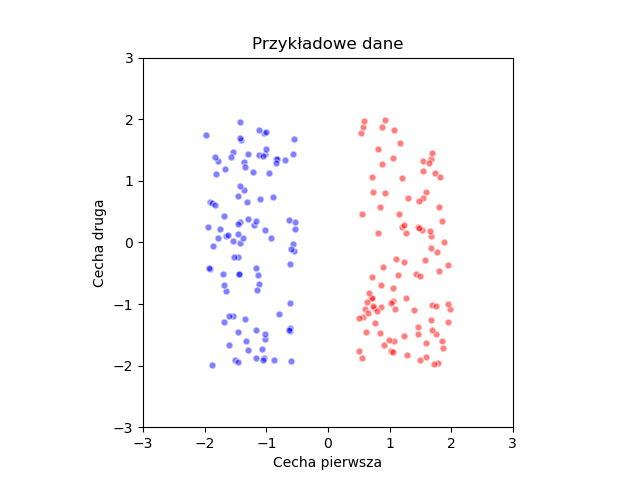
\includegraphics[width=\scaly\textwidth]{images/c0n0_data.png}\end{center}\end{frame}
\begin{frame}\begin{center}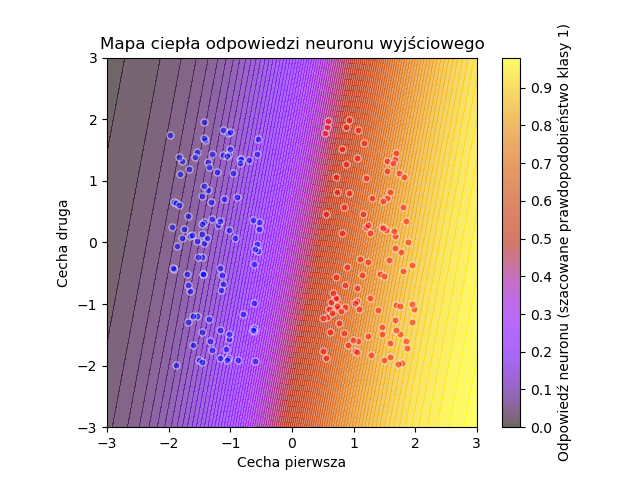
\includegraphics[width=\scaly\textwidth]{images/c0n0_output.png}\end{center}\end{frame}

\begin{frame}\begin{center}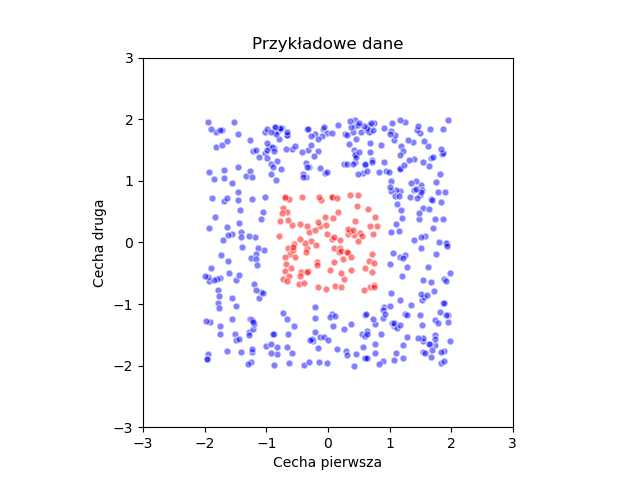
\includegraphics[width=\scaly\textwidth]{images/c1n0r0_data.png}\end{center}\end{frame}
\begin{frame}\begin{center}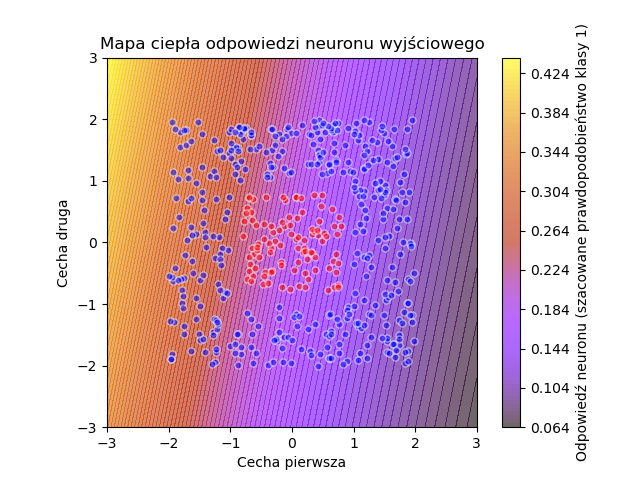
\includegraphics[width=\scaly\textwidth]{images/c1n0r0_output.png}\end{center}\end{frame}
\begin{frame}\begin{center}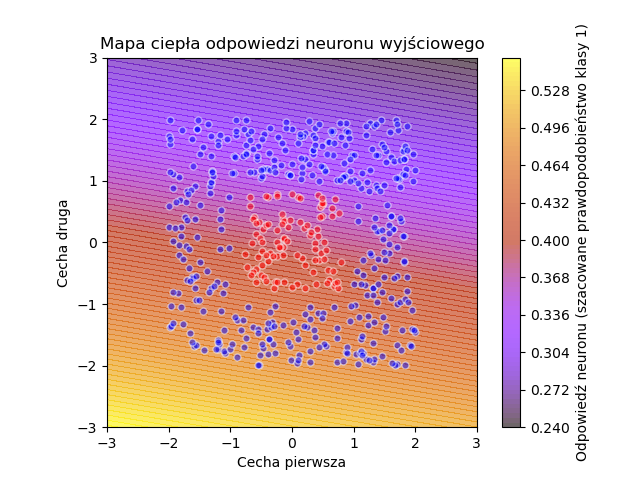
\includegraphics[width=\scaly\textwidth]{images/c1n0r1_output.png}\end{center}\end{frame}

\subsection{Jeden neuron wyjściowy, cztery w warstwie ukrytej $\circledast\circledast \rightarrow \circleddash\circleddash\circleddash\circleddash \rightarrow \circledcirc$}

\begin{frame}\begin{center}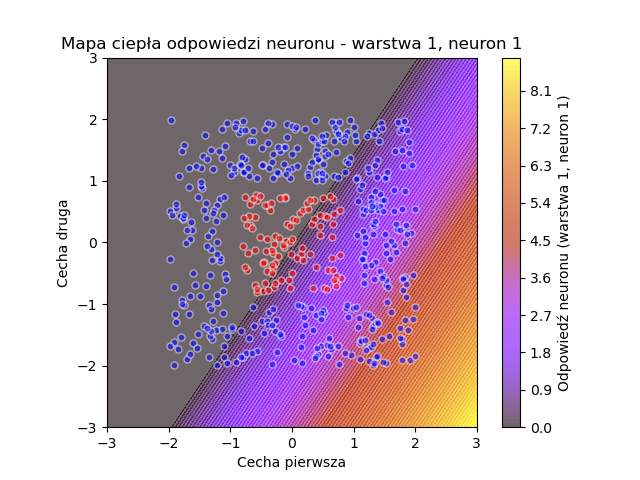
\includegraphics[width=\scaly\textwidth]{images/c1n1_l0_n0.png}\end{center}\end{frame}
\begin{frame}\begin{center}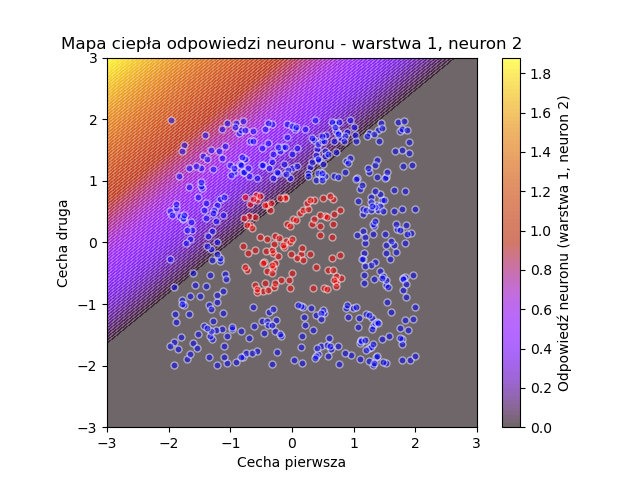
\includegraphics[width=\scaly\textwidth]{images/c1n1_l0_n1.png}\end{center}\end{frame}
\begin{frame}\begin{center}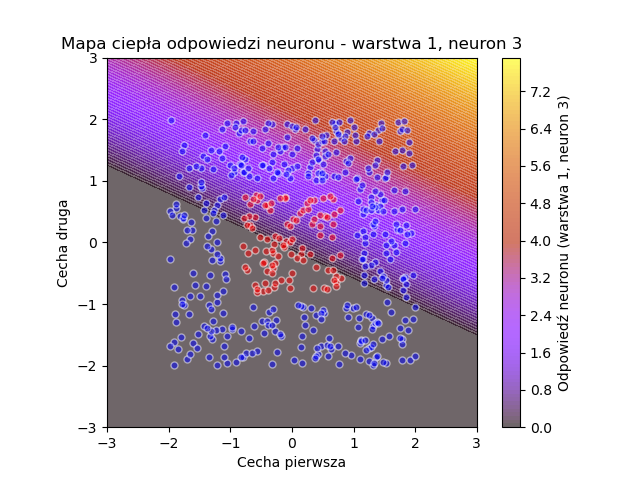
\includegraphics[width=\scaly\textwidth]{images/c1n1_l0_n2.png}\end{center}\end{frame}
\begin{frame}\begin{center}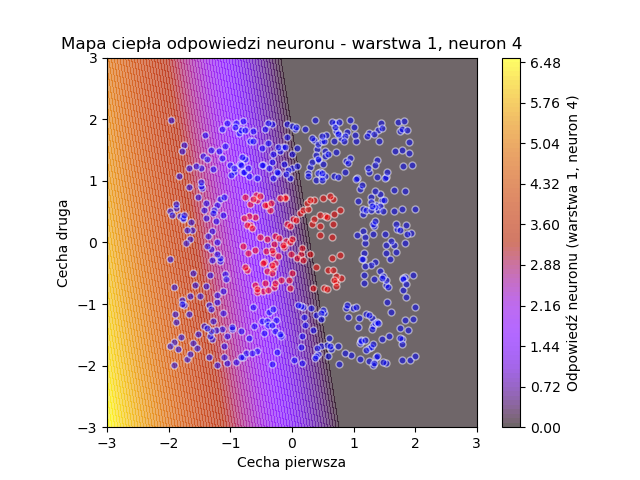
\includegraphics[width=\scaly\textwidth]{images/c1n1_l0_n3.png}\end{center}\end{frame}
\begin{frame}\begin{center}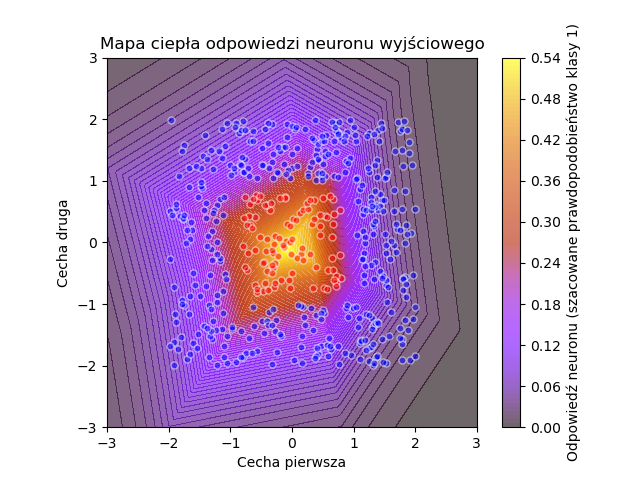
\includegraphics[width=\scaly\textwidth]{images/c1n1_output.png}\end{center}\end{frame}

\begin{frame}\begin{center}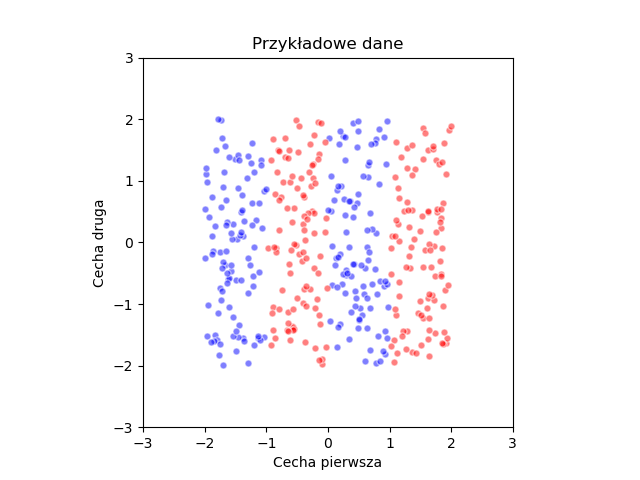
\includegraphics[width=\scaly\textwidth]{images/c2n1_data.png}\end{center}\end{frame}
\begin{frame}\begin{center}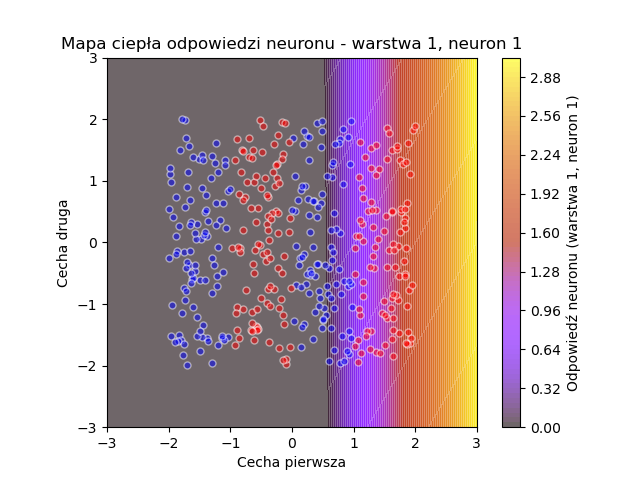
\includegraphics[width=\scaly\textwidth]{images/c2n1_l0_n0.png}\end{center}\end{frame}
\begin{frame}\begin{center}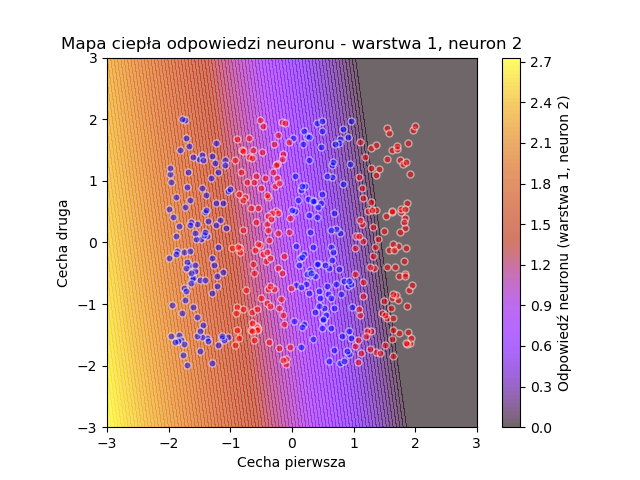
\includegraphics[width=\scaly\textwidth]{images/c2n1_l0_n1.png}\end{center}\end{frame}
\begin{frame}\begin{center}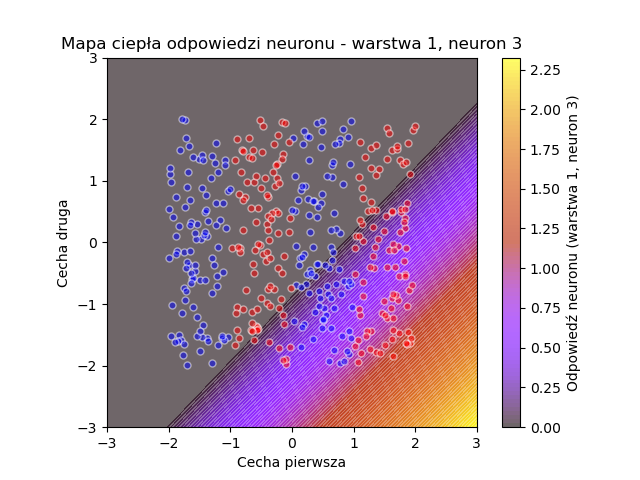
\includegraphics[width=\scaly\textwidth]{images/c2n1_l0_n2.png}\end{center}\end{frame}
\begin{frame}\begin{center}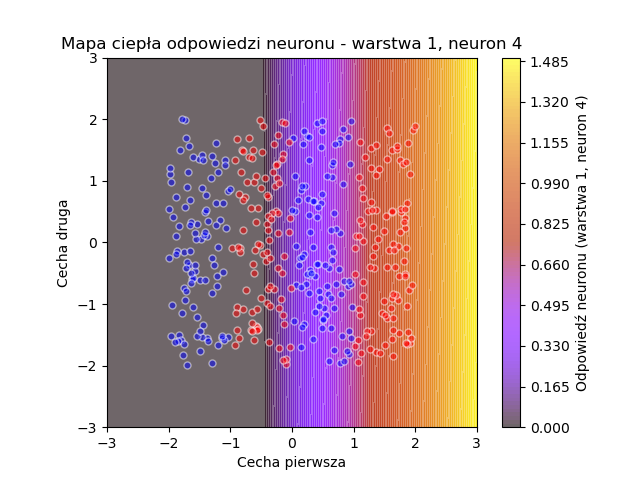
\includegraphics[width=\scaly\textwidth]{images/c2n1_l0_n3.png}\end{center}\end{frame}
\begin{frame}\begin{center}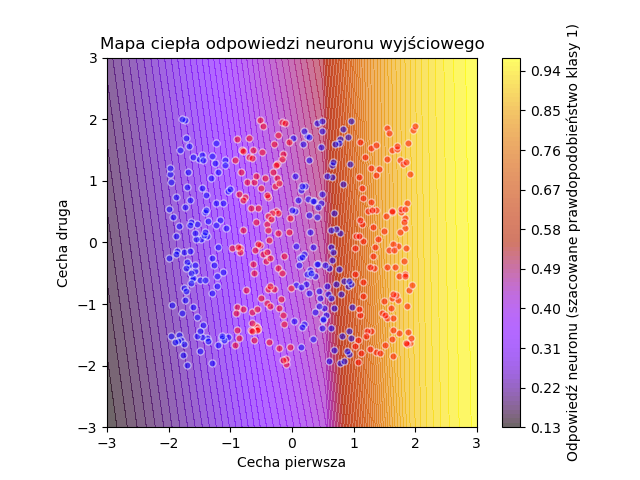
\includegraphics[width=\scaly\textwidth]{images/c2n1_output.png}\end{center}\end{frame}

\subsection{2 warstwy ukryte (5, 5), $\circledast\circledast \rightarrow \circleddash\circleddash\circleddash\circleddash\circleddash \rightarrow \circleddash\circleddash\circleddash\circleddash\circleddash \rightarrow \circledcirc$}

\begin{frame}\begin{center}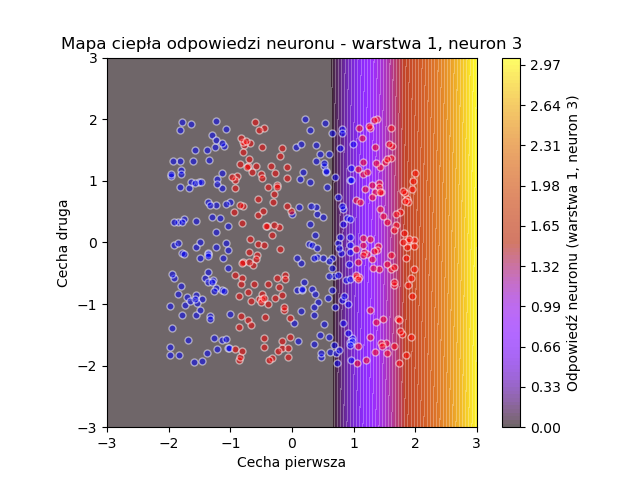
\includegraphics[width=\scaly\textwidth]{images/c2n2_l0_n2.png}\end{center}\end{frame}
\begin{frame}\begin{center}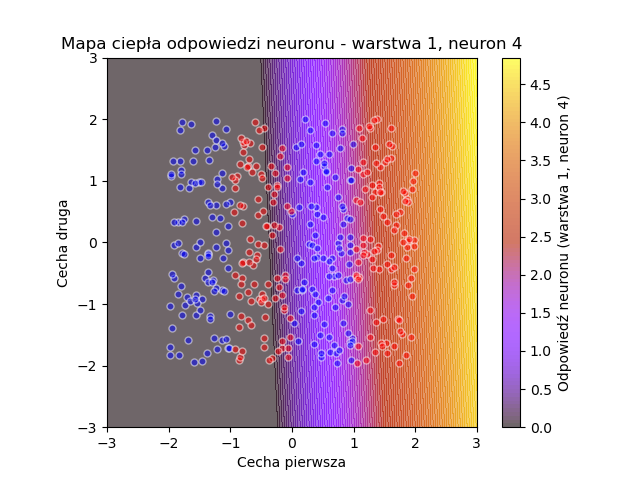
\includegraphics[width=\scaly\textwidth]{images/c2n2_l0_n3.png}\end{center}\end{frame}
\begin{frame}\begin{center}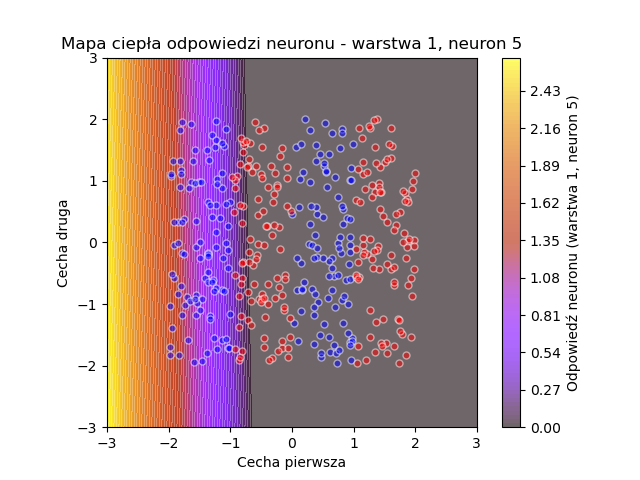
\includegraphics[width=\scaly\textwidth]{images/c2n2_l0_n4.png}\end{center}\end{frame}
\begin{frame}\begin{center}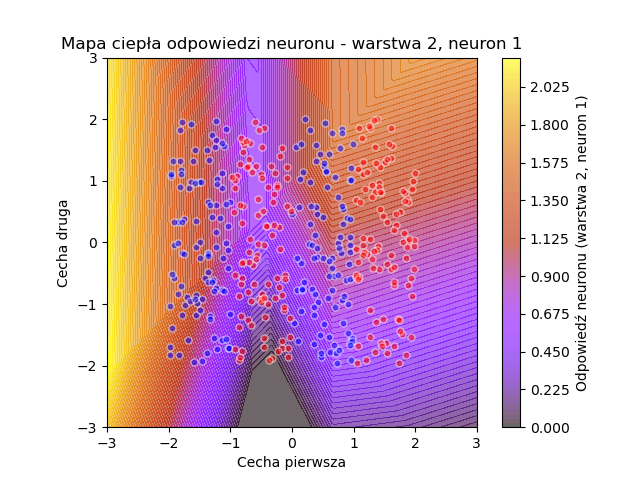
\includegraphics[width=\scaly\textwidth]{images/c2n2_l1_n0.png}\end{center}\end{frame}
\begin{frame}\begin{center}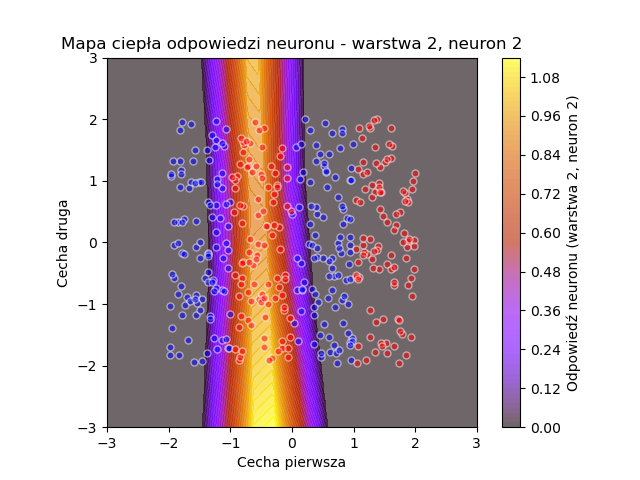
\includegraphics[width=\scaly\textwidth]{images/c2n2_l1_n1.png}\end{center}\end{frame}
\begin{frame}\begin{center}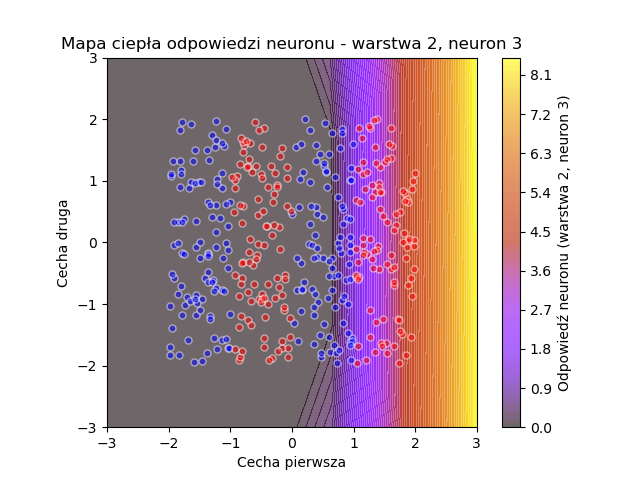
\includegraphics[width=\scaly\textwidth]{images/c2n2_l1_n2.png}\end{center}\end{frame}
\begin{frame}\begin{center}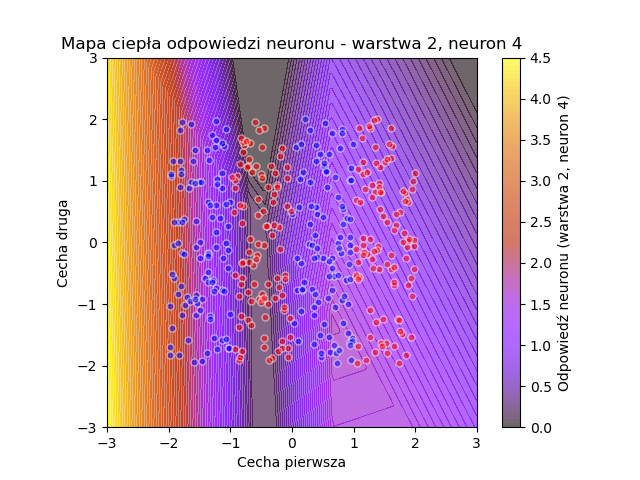
\includegraphics[width=\scaly\textwidth]{images/c2n2_l1_n3.png}\end{center}\end{frame}
\begin{frame}\begin{center}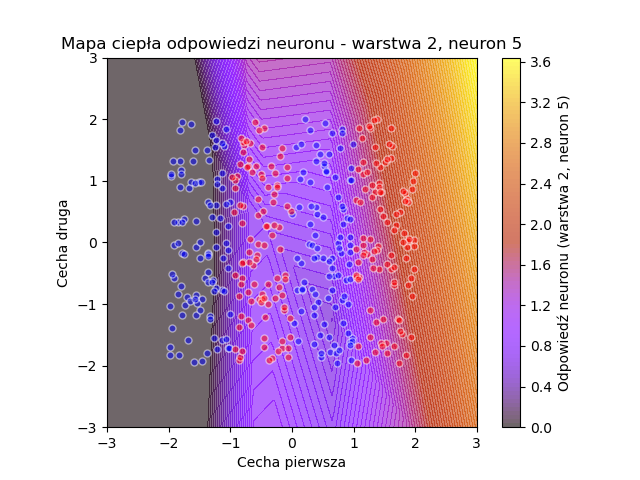
\includegraphics[width=\scaly\textwidth]{images/c2n2_l1_n4.png}\end{center}\end{frame}
\begin{frame}\begin{center}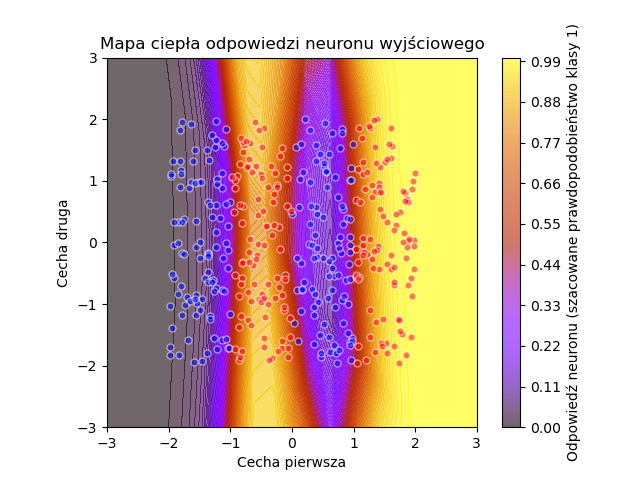
\includegraphics[width=\scaly\textwidth]{images/c2n2_output.png}\end{center}\end{frame}

\begin{frame}\begin{center}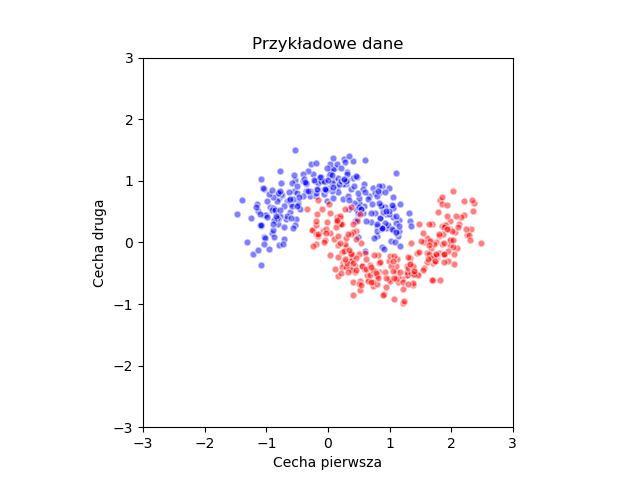
\includegraphics[width=\scaly\textwidth]{images/c3n2_data.png}\end{center}\end{frame}
\begin{frame}\begin{center}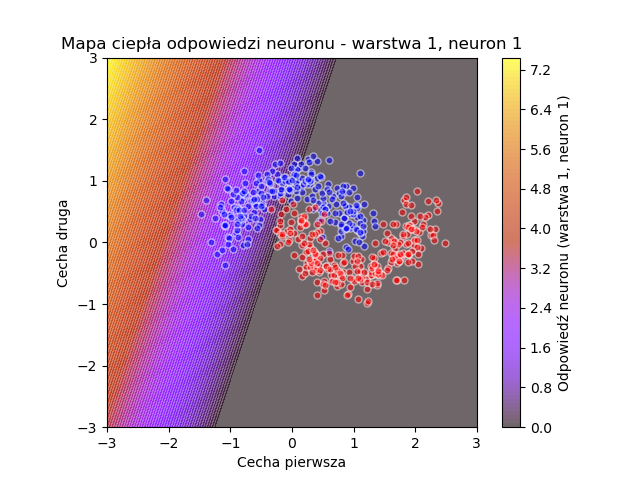
\includegraphics[width=\scaly\textwidth]{images/c3n2_l0_n0.png}\end{center}\end{frame}
\begin{frame}\begin{center}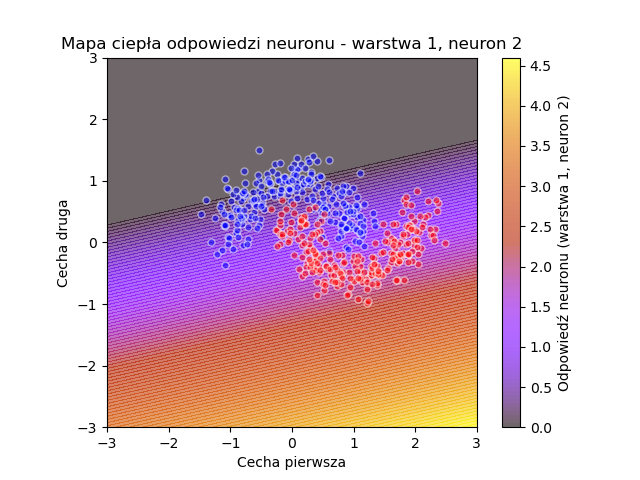
\includegraphics[width=\scaly\textwidth]{images/c3n2_l0_n1.png}\end{center}\end{frame}
\begin{frame}\begin{center}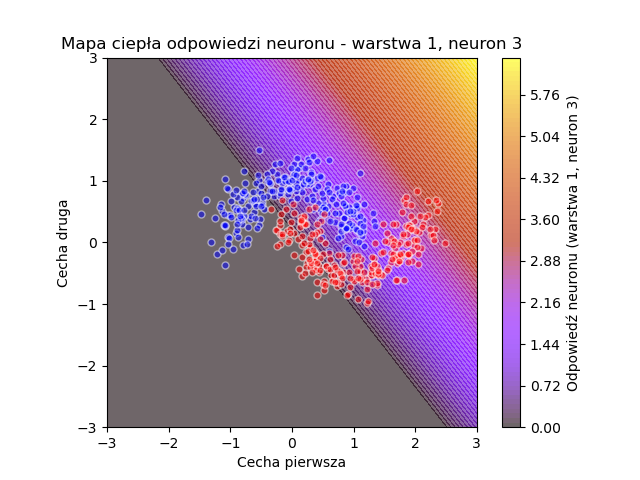
\includegraphics[width=\scaly\textwidth]{images/c3n2_l0_n2.png}\end{center}\end{frame}
\begin{frame}\begin{center}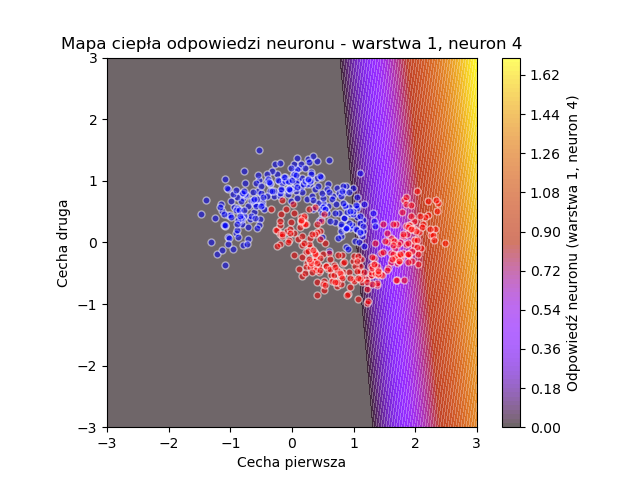
\includegraphics[width=\scaly\textwidth]{images/c3n2_l0_n3.png}\end{center}\end{frame}
\begin{frame}\begin{center}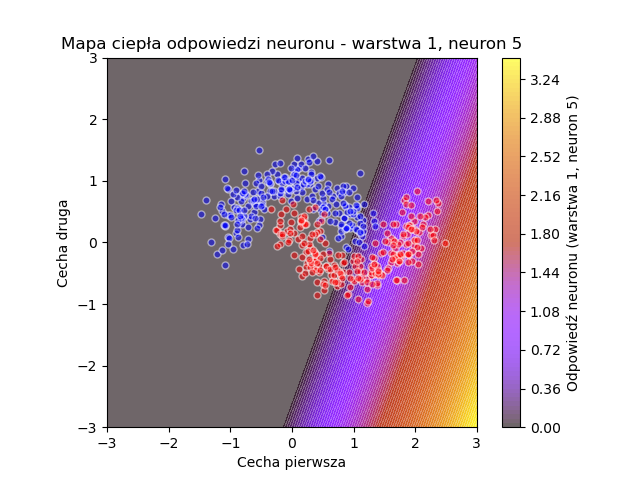
\includegraphics[width=\scaly\textwidth]{images/c3n2_l0_n4.png}\end{center}\end{frame}
\begin{frame}\begin{center}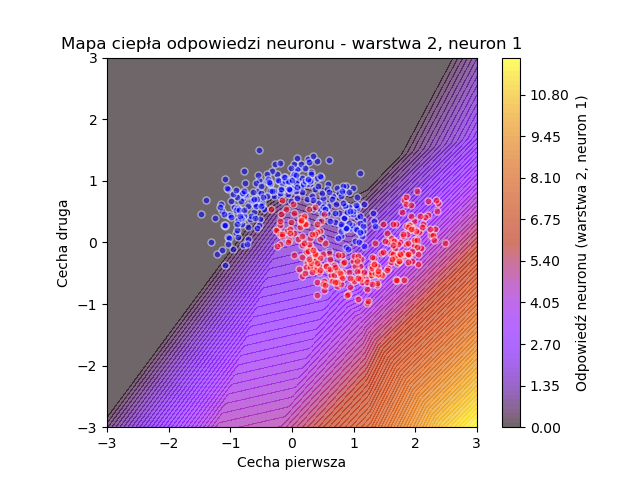
\includegraphics[width=\scaly\textwidth]{images/c3n2_l1_n0.png}\end{center}\end{frame}
\begin{frame}\begin{center}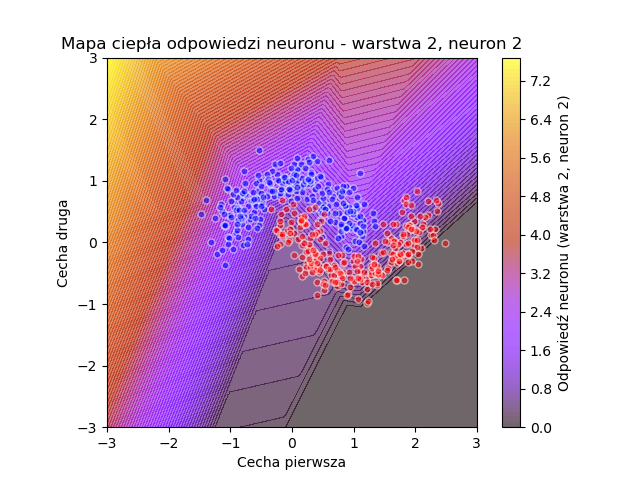
\includegraphics[width=\scaly\textwidth]{images/c3n2_l1_n1.png}\end{center}\end{frame}
%\begin{frame}\begin{center}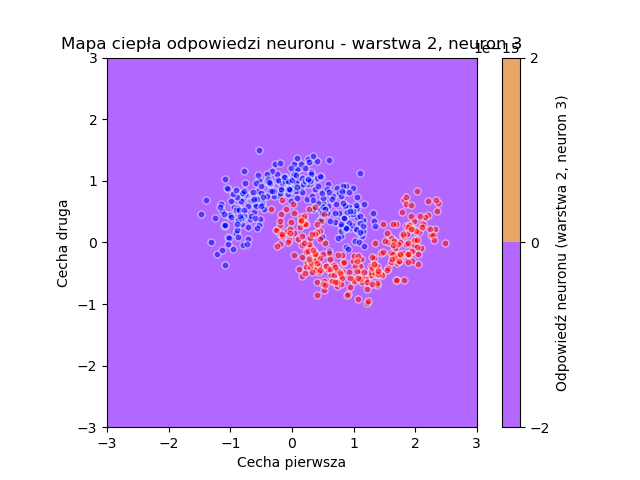
\includegraphics[width=\scaly\textwidth]{images/c3n2_l1_n2.png}\end{center}\end{frame}
\begin{frame}\begin{center}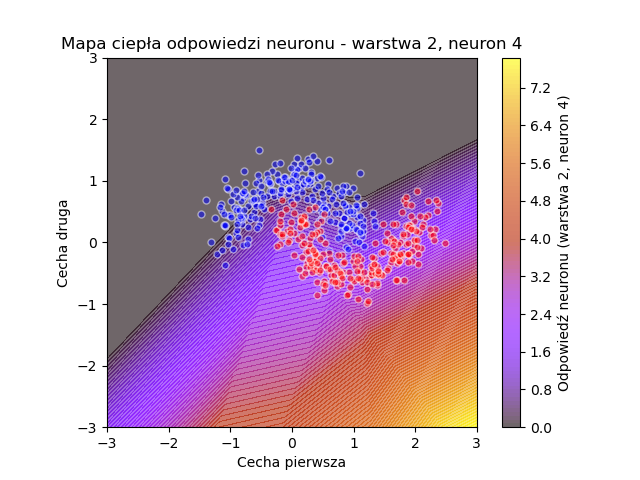
\includegraphics[width=\scaly\textwidth]{images/c3n2_l1_n3.png}\end{center}\end{frame}
%\begin{frame}\begin{center}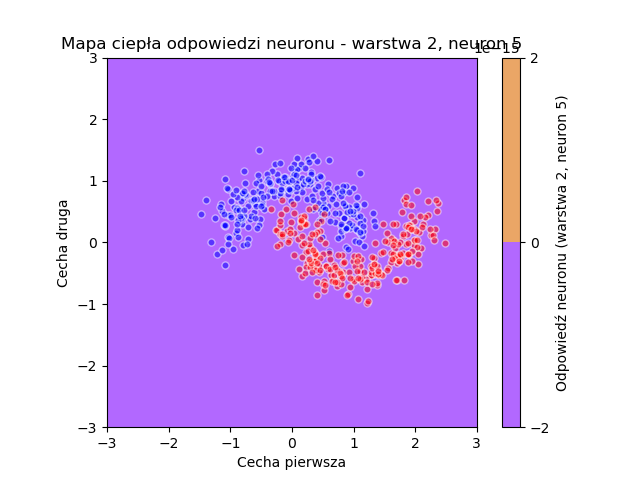
\includegraphics[width=\scaly\textwidth]{images/c3n2_l1_n4.png}\end{center}\end{frame}
\begin{frame}\begin{center}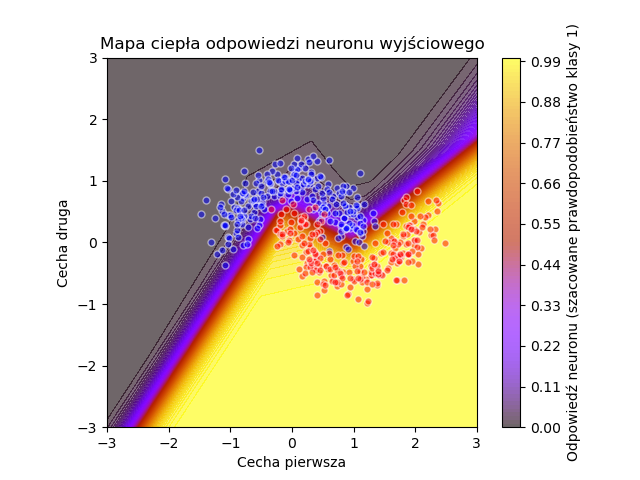
\includegraphics[width=\scaly\textwidth]{images/c3n2_output.png}\end{center}\end{frame}

\subsection{2 warstwy ukryte (10, 10), $\circledast\circledast \rightarrow 10 \times \circleddash \rightarrow 10 \times \circleddash \rightarrow \circledcirc$}

\begin{frame}\begin{center}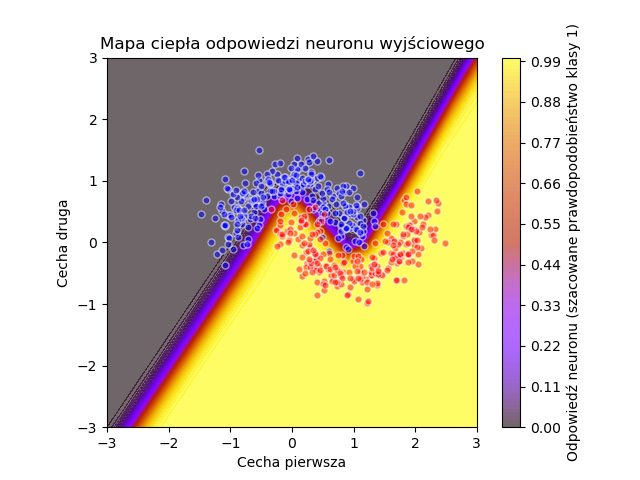
\includegraphics[width=\scaly\textwidth]{images/c3nX_output.png}\end{center}\end{frame}
\begin{frame}\begin{center}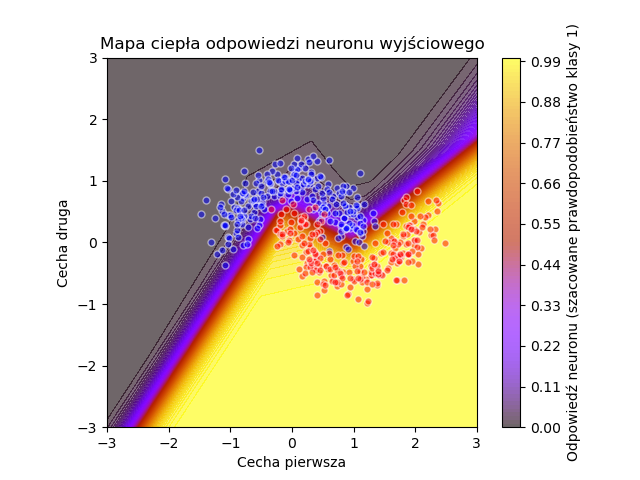
\includegraphics[width=0.45\textwidth]{images/c3n2_output.png}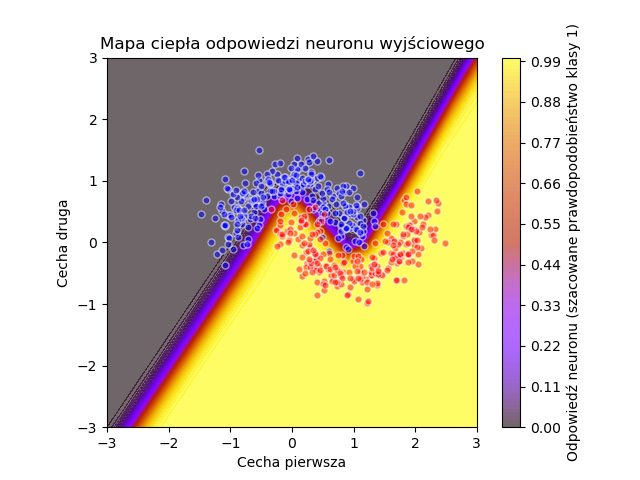
\includegraphics[width=0.45\textwidth]{images/c3nX_output.png}\end{center}\end{frame}

\end{document}


%\section{Sekcja 1}
%\subsection{Podsekcja 1}
%\subsubsection{Podpodsekcja 1}
%
%\begin{frame}{Tytuł slajdu}
%	\framesubtitle{Podtytuł slajdu}
%	\begin{itemize}
%		\item \lipsum[1]
%	\end{itemize}
%\end{frame}
%
%\begin{frame}{Tytuł slajdu}
%	\begin{block}{Tytuł bloku}
%		\lipsum[1]
%	\end{block}
%\end{frame}
%
%\begin{frame}{Tytuł slajdu}
%	\begin{theorem}
%		$\ket{x}=[0,1]^\dagger$
%	\end{theorem}
%\end{frame}
%
%\begin{frame}{Tytuł slajdu}
%	\begin{exampleblock}{Przykład 1}
%		$\ket{x}=[0,1]^\dagger$
%	\end{exampleblock}
%\end{frame}
